\begin{tabular}{M{6.5cm}M{11cm}}
	\textbf{TRUNG TÂM MANABIE}& \textbf{ĐỀ ÔN TẬP KIỂM TRA GIỮA HỌC KÌ 1}\\
	\textbf{MÃ ĐỀ: 004}& \textbf{Bài thi môn: VẬT LÝ 12}\\
	\textit{(Đề trường Nguyễn Khuyến TpHCM\newline năm học 2024 -2025)}& \textit{Thời gian làm bài: 50 phút, không kể thời gian phát đề}
	
	\noindent\rule{4cm}{0.8pt} \\
\end{tabular}
\setcounter{section}{0}
\section{Câu trắc nghiệm nhiều phương án lựa chọn}
\textit{Thí sinh trả lời từ câu 1 đến câu 18. Mỗi câu hỏi thí sinh chọn một phương án}
\setcounter{ex}{0}
\Opensolutionfile{ans}[ans/G12-4-TN]
% ===================================================================
\begin{ex}
	Nhiệt dung riêng của một chất là nhiệt lượng cần thiết để làm cho
	\choice
	{$\SI{1}{\meter^3}$ chất đó tăng thêm $\SI{1}{\celsius}$}
	{$\SI{1}{\kilogram}$ chất đó tăng thêm $\SI{100}{\celsius}$}
	{\True $\SI{1}{\kilogram}$ chất đó tăng thêm $\SI{1}{\celsius}$}
	{$\SI{1}{\meter^3}$ chất đó tan chảy hoàn toàn}
	\loigiai{}
\end{ex}
% ===================================================================
\begin{ex}
Cách làm thay đổi nội năng chủ yếu bằng hình thức thực hiện công cơ học là	
	\choice
	{bỏ miếng kim loại vào nước đá}
	{bỏ miếng kim loại vào nước nóng}
	{hơ nóng miếng kim loại trên ngọn lửa đèn cồn}
	{\True ma sát (chà) một miếng kim loại trên mặt bàn}
	\loigiai{}
\end{ex}
% ===================================================================
\begin{ex}
	Chuyển động của các phân tử, nguyên tử được gọi là
	\choice
	{dao động cơ}
	{dao động điều hòa}
	{\True chuyển động nhiệt}
	{chuyển động từ}
	\loigiai{}
\end{ex}
% ===================================================================
\begin{ex}
	Nhiệt độ âm trong thang nhiệt độ Celsius là nhiệt độ
	\choice
	{tan chảy của nước đá}
	{\True thấp hơn $\SI{0}{\celsius}$}
	{từ $\SI{35}{\celsius}$ đến $\SI{42}{\celsius}$}
	{từ $\SI{0}{\celsius}$ đến $\SI{100}{\celsius}$}
	\loigiai{}
\end{ex}
% ===================================================================
\begin{ex}
	Gọi $m$ là khối lượng của một phân tử của một chất khí. Biết khối khí này có $N$ phân tử, thể tích là $V$. Khối lượng riêng của chất khí này là
	\choice
	{$\dfrac{V}{Nm}$}
	{\True $\dfrac{Nm}{V}$}
	{$\dfrac{m}{NV}$}
	{$\dfrac{m}{V}$}
	\loigiai{}
\end{ex}
% ===================================================================
\begin{ex}
Một số chất ở thể rắn như iodine, băng phiến, đá khô,\dots có thể chuyển trực tiếp sang \dots (1) 
\dots khi nó \dots (2) \dots Hiện tượng trên gọi là sự thăng hoa. Ngược lại với sự thăng hoa là sự ngưng kết. Điền cụm từ thích hợp vào chố trống.	
	\choice
	{(1) thể lỏng; (2) nhận nhiệt}
	{\True (1) thể hơi; (2) nhận nhiệt}
	{(1) thể lỏng; (2) tỏa nhiệt}
	{(1) thể hơi; (2) tỏa nhiệt}
	\loigiai{}
\end{ex} %===================================================================
%
\begin{ex}
	Trong hệ SI, đơn vị của nhiệt nóng chảy riêng là
	\choice
	{\True $\si{\joule/\kilogram}$}
	{$\si{cal}$}
	{$\si{\electronvolt}$}
	{$\si{\joule}$}
	\loigiai{}
\end{ex}
% ===================================================================
\begin{ex}
	Điều nào sau đây là \textbf{sai} khi nói về nội năng?
	\choice
	{\True Nội năng không thể biến đổi được}
	{Nội năng của một vật phụ thuộc vào nhiệt độ và thể tích của vật}
	{Đơn vị của nội năng là Jun ($\si{\joule}$)}
	{Nội năng của một vật là dạng năng lượng bao gồm tổng động năng của các phân tử cấu tạo nên vật và thế năng tương tác giữa chúng}
	\loigiai{}
\end{ex}
% ===================================================================
\begin{ex}
Hai vật rắn (1) và (2) tiếp xúc nhau. Vật (1) đang có nhiệt độ cao hơn vật (2). Phát biểu nào sau đây \textbf{không} chính xác?	
	\choice
	{\True Vật (1) có nội năng lớn hơn vật (2)}
	{Năng lượng nhiệt được truyền từ vật (1) sang vật (2)}
	{Tốc độ trung bình của các phân tử trong vật (1) cao hơn tốc độ trung bình của các phân tử trong vật (2)}
	{Quá trình truyền nhiệt giữa 2 vật dừng lại khi chúng có nhiệt độ bằng nhau}
	\loigiai{
	Nội năng của 1 hệ phụ thuộc nhiệt độ và thể tích của hệ, nhiệt độ hệ (1) cao hơn hệ (2) chưa chắc nội năng hệ (1) lớn hơn nội năng hệ (2).
	}
\end{ex}
% ===================================================================
\begin{ex}
	Tính chất nào sau đây \textbf{không phải} của nguyên tử, phân tử?
	\choice
	{\True Nở ra khi nhiệt độ tăng, co lại khi nhiệt độ giảm}
	{Chuyển động càng nhanh khi nhiệt độ càng cao}
	{Giữa chúng có khoảng cách}
	{Chuyển động không ngừng}
	\loigiai{}
\end{ex}
% ===================================================================
\begin{ex}
Trong các chất sau, chất nào không phải là chất rắn kết tinh?	
	\choice
	{Nước đá}
	{Muối ăn}
	{Kim cương}
	{\True Nhựa đường}
	\loigiai{}
\end{ex}
% ===================================================================
\begin{ex}
	Tính chất nào sau đây \textbf{không phải} là tính chất của chất ở thể khí?
	\choice
	{Có thể nén được dễ dàng}
	{\True Có hình dạng và thể tích riêng}
	{Có các phân tử chuyển động hỗn độn}
	{Có lực tương tác phân tử nhỏ hơn lực tương tác phân tử ở thể rắn và thể lỏng}
	\loigiai{}
\end{ex}
% ===================================================================
\begin{ex}
	Bảng dưới đây cho biết nhiệt độ nóng chảy và nhiệt độ sôi của một số chất
	\begin{center}
		\begin{tabular}{|M{5cm}|M{5cm}|M{5cm}|}
		\hline
		\thead{Chất}&\thead{Nhiệt độ nóng chảy $\left(\si{\celsius}\right)$} &\thead{Nhiệt độ sôi $\left(\si{\celsius}\right)$}\\
		\hline
		1&$\SI{-201}{}$&$\SI{-196}{}$\\
		\hline
		2&$\SI{-39}{}$&357\\
		\hline
		3&30&2400\\
		\hline
		4&327&1749\\
		\hline
		\end{tabular}
	\end{center}
	Chất nào ở thể lỏng ở $\SI{20}{\celsius}$?
	\choice
	{\True Chất 2}
	{Chất 1}
	{Chất 3}
	{Chất 4}
	\loigiai{}
\end{ex}
% ===================================================================
\begin{ex}
	Hình dưới đây biểu diễn sự thay đổi nhiệt độ theo thời gian của chất A
	\begin{center}
		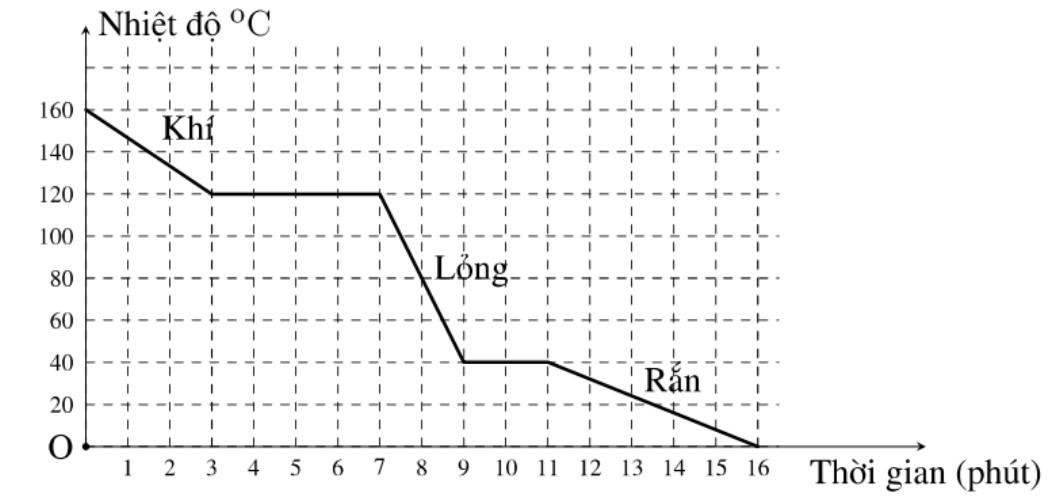
\includegraphics[width=0.7\linewidth]{../figs/D12-4-1}
	\end{center}
	Nhận xét nào sau đây \textbf{không đúng}?
	\choice
	{Nhiệt độ sôi của chất A là $\SI{120}{\celsius}$}
	{\True Ở phút thứ 8 , chất A tồn tại ở cả 3 thể rắn, lỏng và khí (hơi)}
	{Nhiệt độ nóng chảy của chất A là $\SI{40}{\celsius}$}
	{Ở phút thứ 4 , chất A đang ngưng tụ}
	\loigiai{
	Ở phút thứ 8 chất này chỉ tồn tại ở thể lỏng.
	}
\end{ex}
% ===================================================================
\begin{ex}
	Ở nhiệt độ bao nhiêu trong thang Celsius thì giá trị nhiệt độ bằng một nửa nhiệt độ tuyệt đối của nó?
	\choice
	{$\SI{50}{\celsius}$}
	{$\SI{0}{\celsius}$}
	{$\SI{100}{\celsius}$}
	{\True $\SI{273}{\celsius}$}
	\loigiai{
	$$t=\dfrac{t+273}{2}\Rightarrow t=\SI{273}{\celsius}.$$
	}
\end{ex}
% ===================================================================
\begin{ex}
	Một khối khí dãn nở thêm 1 lít ở áp suất không đổi là $\SI{E5}{\newton/\meter^2}$. Trong quá trình này, khối khí nhận thêm nhiệt lượng là $\SI{500}{\joule}$. Độ biến thiên nội năng của khí là
	\choice
	{$\SI{600}{\joule}$}
	{$\SI{-600}{\joule}$}
{\True $\SI{400}{\joule}$}
	{$\SI{-400}{\joule}$}
	\loigiai{
	Công khối khí thực hiện:
	$$A'=p\Delta V=\left(\SI{E5}{\newton/\meter^2}\right)\cdot\left(\SI{1E-3}{\meter^3}\right)=\SI{100}{\joule}.$$
	Độ biến thiên nội năng của khí:
	$$\Delta U=Q+A=Q-A'=\SI{400}{\joule}.$$
	}
\end{ex}
% ===================================================================
\begin{ex}
	Nhiệt lượng cần cung cấp để một khối băng có khối lượng $\SI{2}{\kilogram}$ tan chảy hoàn toàn ở nhiệt độ tan chảy $\SI{0}{\celsius}$ là $\SI{666}{\kilo\joule}$. Nhiệt nóng chảy riêng của băng bằng
	\choice
	{$\SI{68}{\kilo\joule/\kilogram}$}
	{\True $\SI{333}{\kilo\joule/\kilogram}$}
	{$\SI{136}{\kilo\joule/\kilogram}$}
	{$\SI{170}{\kilo\joule/\kilogram}$}
	\loigiai{
	$$\lambda=\dfrac{Q}{m}=\SI{333}{\kilo\joule/\kilogram}.$$
	}
\end{ex}
% ===================================================================
\begin{ex}
	Biết nhiệt hóa hơi riêng của nước ở $\SI{100}{\celsius}$ là $\SI{2.26E6}{\joule/\kilogram}$. Nhiệt lượng cần thiết để chuyển $\SI{2.5}{\kilogram}$ nước ở $\SI{100}{\celsius}$ thành hơi hoàn toàn là
	\choice
	{\True $\SI{5650}{\kilo\joule}$}
	{$\SI{904}{\kilo\joule}$}
	{$\SI{904}{\joule}$}
	{$\SI{5650}{\joule}$}
	\loigiai{
	$$Q=mL=\left(\SI{2.5}{\kilogram}\right)\cdot\left(\SI{2.26E6}{\joule/\kilogram}\right)=\SI{5650}{\kilo\joule}.$$
	}
\end{ex}
\Closesolutionfile{ans}
\section{Câu trắc nghiệm đúng/sai} 
\textit{Thí sinh trả lời từ câu 1 đến câu 4. Trong mỗi ý \textbf{a)}, \textbf{b)}, \textbf{c)}, \textbf{d)} ở mỗi câu, thí sinh chọn đúng hoặc sai}
\setcounter{ex}{0}
\Opensolutionfile{ans}[ans/G12-4-TF]
% ===================================================================
\begin{ex}
	\immini{
	Một lượng khí chứa trong một xilanh có pittông di chuyển được. Ở trạng thái cân bằng, chất khí chiếm thể tích $V\left(\si{\meter^3}\right)$ và tác dụng lên pittông một áp suất $\SI{4E5}{\newton/\meter^2}$. Khối khí nhận một nhiệt lượng $\SI{1000}{\joule}$ giãn nở đẩy pittông lên làm thể tích khí tăng thêm $\SI{0.003}{\meter^3}$. Coi rằng áp suất chất khí không đổi.
	}
	{
	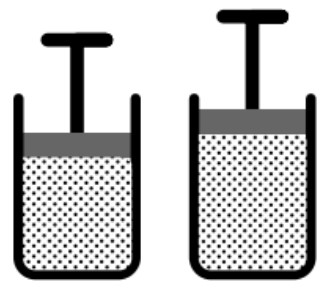
\includegraphics[width=0.4\linewidth]{../figs/D12-4-2}
	}
	\choiceTF[t]
	{Theo quy ước, khối khí nhận nhiệt và sinh công nên $A>0$; $A>0$}
	{\True Độ biến thiên nội năng của khối khí $\Delta U=\SI{-200}{\joule}$}
	{\True Công mà khối khí thực hiện có độ lớn bằng $\SI{1200}{\joule}$}
	{\True Lượng khí bên trong xilanh nhận nhiệt và sinh công làm biến đổi nội năng}
	\loigiai{
	\begin{itemchoice}
		\itemch Sai. $Q>0$, $A<0$.
		\itemch Đúng. $\Delta U=Q-A'=Q-p\Delta V=\SI{-200}{\joule}$.
		\itemch Đúng. $A'=p\Delta V=\SI{1200}{\joule}$.
		\itemch Đúng.
	\end{itemchoice}
	}
\end{ex}
% ===================================================================
\begin{ex}
	Một lượng khí chứa trong một bình thép kín được nung nóng. Bỏ qua sự thay đổi thể tích của bình chứa.
	\choiceTF[t]
	{\True Nếu mỗi phân tử khí có khối lượng $\SI{3.3E-26}{\kilogram}$; bình có thể tích $\SI{20}{\centi\meter^3}$ và số phân tử khí trong bình là $10^{21}$ thì khối lượng riêng của chất khí là $\SI{16.5E-6}{\kilogram/\centi\meter^3}$}
	{Khối lượng riêng của chất khí trong bình tăng lên}
	{Mật độ phân tử khí trong bình tăng lên}
	{\True Tốc độ chuyển động trung bình của các phân tử khí tăng lên}
	\loigiai{
	\begin{itemchoice}
		\itemch Đúng. $D=\dfrac{Nm}{V}=\SI{1.65E-6}{\kilogram/\centi\meter^3}$.
		\itemch Sai.  $N, m, V$ không đổi nên $D$ không đổi.
		\itemch Sai. $N, V$ không đổi nên mật độ phân tử khí $\mu=\dfrac{N}{V}$ không đổi.
		\itemch Đúng. Nhiệt độ tăng nên tốc độ chuyển động nhiệt của các phân tử khí tăng.
	\end{itemchoice}
	}
\end{ex}
% ===================================================================
\begin{ex}
	 Hai vật rắn A và B được làm bằng hai kim loại khác nhau nhưng có cùng khối lượng và được nung nóng đều đặn trong các điều kiện giống nhau. Nhiệt độ của mỗi vật theo thời gian được mô tả bởi đồ thị ở hình bên.
	 \begin{center}
	 	\begin{tikzpicture}  
	 		\begin{axis}[  ultra thick,yscale=0.75,
	 			xmin=0,  
	 			xmax=9,  
	 			xtick={0,1,...,8},
	 			ytick={0,30,...,150},
	 			minor x tick num=0,
	 			minor y tick num=0,
	 			ymin=0,  
	 			ymax=170, 
	 			samples=300,
	 			axis lines=center, 
	 			grid style={step=1, line width =0.6pt, color=gray!50!white},
	 			grid=both, %giới hạn ô lưới
	 			major grid style={line width=0.8pt,gray!85!white},
	 			xlabel=$\xsi{t}{\left(\si{\second}\right)}$, 		ylabel=$\text{Nhiệt độ}\ \si{\celsius}$,
	 			every axis y label/.style={at=(current axis.above origin),anchor=south},  
	 			every axis x label/.style={at=(current axis.right of origin),anchor=west},  ]
	 			\addplot [line width=2pt, red, smooth, domain=0:3] {40*x} node[above left] {A};  
	 			\addplot [line width=2pt, blue, smooth, domain=0:6] {15*x} node[above left] {B}; 
	 			\coordinate (O) at (0,0);
	 		\end{axis}  
	 		\node[below left] at (O) {O};
	 	\end{tikzpicture}
	 \end{center}
	\choiceTF[t]
	{\True Tốc độ tăng nhiệt độ của vật A nhanh hơn tốc độ tăng nhiệt độ của vật B}
	{Ở giây thứ 2 , nhiệt độ của vật A bằng $\SI{78}{\celsius}$}
	{\True Ở giây thứ 2 nhiệt độ của vật B bằng $\SI{30}{\celsius}$}
	{\True Tỉ số nhiệt dung riêng của kim loại A so với nhiệt dung riêng của kim loại B là 0,375}
	\loigiai{
	\begin{itemchoice}
		\itemch Đúng.
		\itemch Sai. $t=\dfrac{2}{3}t_A=\dfrac{2}{3}\cdot120=\SI{80}{\celsius}$.
		\itemch Đúng. 
		\itemch Sai. $\calP=\dfrac{mc_A\cdot120}{3}=\dfrac{mc_B\cdot90}{6}\Rightarrow \dfrac{c_A}{c_B}=0,375.$
	\end{itemchoice}
	}
\end{ex}
% ===================================================================
\begin{ex}
	Một khối nước đá tinh khiết có khối lượng $m=\SI{800}{\gram}$ ở $\SI{-10}{\celsius}$. Biết nhiệt dung riêng của nước đá là $c_{1}=\SI{2090}{\joule/\kilogram\cdot\kelvin}$; nhiệt nóng chảy riêng của nước đá $\lambda=\SI{3.33E5}{\joule/\kilogram}$.
	\choiceTF[t]
	{Khi nước đá tan chảy nó tỏa nhiệt lượng ra môi trường}
	{\True Nhiệt lượng cần thiết để làm cho khối nước đá tăng từ  $\SI{-10}{\celsius}$ lên đến $\SI{0}{\celsius}$ bằng $\SI{16720}{\joule}$}
	{\True Để khối nước đá ở trạng thái trên nóng chảy hoàn toàn thành thể lỏng thì cần một nhiệt lượng tối thiểu là $\SI{283.12}{\kilo\joule}$}
	{\True Ở điều kiện tiêu chuẩn, nước đá tinh khiết nóng chảy ở $\SI{0}{\celsius}$}
	\loigiai{
	
	}
\end{ex}
\Closesolutionfile{ans}
\section{Câu trắc nghiệm trả lời ngắn} \textit{Thí sinh trả lời từ câu 1 đến câu 6}
\setcounter{ex}{0}
\Opensolutionfile{ans}[ans/G12-4-TL]
% ===============================================================
\begin{ex}
	Biết nhiệt nóng chảy riêng của nước đá là $\lambda=\SI{34E4}{\joule/\kilogram}$ và nhiệt dung riêng của nước là $\SI{4180}{\joule/\kilogram\cdot\kelvin}$. Nhiệt lượng cần cung cấp cho $\SI{4}{\kilogram}$ nước đá ở $\SI{0}{\celsius}$ để chuyển nó thành nước $\SI{20}{\celsius}$ là bao nhiêu $\si{\kilo\joule}$? \textit{(Làm tròn đến phần nguyên của kết quả)}
	\shortans{1694}
	\loigiai{
		$$Q=m\left(\lambda+ct\right)=\SI{1694400}{\joule}\approx\SI{1694}{\kilo\joule}.$$
	}
\end{ex}
% ===============================================================
\begin{ex}
	Biết nhiệt dung riêng của nước đá là $c_{1}=\SI{2100}{\joule/\kilogram\cdot\kelvin}$, nhiệt dung riêng của nước là $c_{2}=\SI{4200}{\joule/\kilogram\cdot\kelvin}$. Để tìm nhiệt nóng chảy riêng của nước đá, người ta làm thí nghiệm như sau: Dùng một bếp điện để đun một hệ gồm một bình bằng đồng đựng một lượng nước đá với nhiệt độ ban đầu của hệ là $\SI{-5}{\celsius}$. Dùng nhiệt kế để đo nhiệt độ của hệ, người ta thu được bảng sau:
	\begin{center}
		\begin{tabular}{|M{3cm}|M{1.5cm}|M{1.5cm}|M{1.5cm}|M{1.5cm}|M{1.5cm}|M{1.5cm}|M{1.5cm}|M{1.5cm}|}
		\hline
		\thead{Thời gian $\left(\si{\second}\right)$} & 0& 60 & 360 & 660 & 960 & 1260 &1340 & 1540\\
		\hline
		\thead{Nhiệt độ $\left(\si{\celsius}\right)$}& $\SI{-5}{}$ & 0&0&0&0&0&0&10\\
		\hline
		\end{tabular}
	\end{center}
	Biết rằng từ thời điểm 0 đến $\SI{60}{\second}$ và $\SI{1340}{\second}$ đến $\SI{1540}{\second}$, số chỉ của nhiệt kế tăng liên tục. Coi như nhiệt lượng mà hệ nhận được tỉ lệ với thời gian đun (hệ số tỉ lệ không đổi). Nhiệt nóng chảy riêng của nước đá đo được trong thí nghiệm này là $\xsi{x\cdot10^5}{\joule/\kilogram}$. Giá trị của $x$ bằng bao nhiêu?
	\shortans{3,36 }
	\loigiai{
		Gọi $m$ và $m_b$ lần lượt là khối lượng của nước đá và khối lượng của bình.\\
		$$\begin{cases}
			\calP\cdot60=\left(mc_1+m_bc_b\right)\cdot 5\\
			\calP\cdot\left(1340-60\right)=m\lambda\\
			\calP\cdot\left(1540-1340\right)=\left(mc_2+m_bc_b\right)\cdot10
		\end{cases}\Rightarrow \begin{cases}
		\dfrac{m}{\calP}\cdot2100+\dfrac{m_bc_b}{\calP}=\dfrac{60}{5}\\
		\dfrac{m\lambda}{\calP}=1340-60\\
		\dfrac{m}{\calP}\cdot4200+\dfrac{m_bc_b}{\calP}=\dfrac{1540-1340}{10}
		\end{cases}\Rightarrow\begin{cases}
		\dfrac{m}{\calP}=\dfrac{2}{525}\\
		\lambda=\SI{3.36E5}{\joule/\kilogram}\\
		\dfrac{m_bc_b}{\calP}=4
		\end{cases}.$$
	}
\end{ex}
% ===============================================================
\begin{ex}
	Trong một bình nhiệt lượng kế có chứa $\SI{200}{\milli\liter}$ nước ở nhiệt độ ban đầu $t_{0}=\SI{10}{\celsius}$. Người ta dùng một cốc đổ $\SI{50}{\milli\liter}$ nước ở nhiệt độ $\SI{60}{\celsius}$ vào bình rồi sau khi cân bằng nhiệt lại múc ra từ bình $\SI{50}{\milli\liter}$ nước. Bỏ qua sự trao đổi nhiệt với cốc bình và môi trường. Hỏi sau tối thiểu bao nhiêu lượt đổ thì nhiệt độ của nước trong bình sẽ lớn hơn $\SI{40}{\celsius}$? 
	\textit{(Một lượt đổ gồm một lần múc nước vào và một lần múc nước ra).}
	\shortans{5}
	\loigiai{
		Sau $n$ lượt đổ thì nhiệt độ cân bằng là
		$$t_n=\dfrac{m_0t_{n-1}+t\Delta m}{m_0+\Delta m}=\dfrac{200t_{n-1}+50\cdot60}{200+50}.$$
		Chạy vòng lặp:
		$$A=A+1:X=\dfrac{200X+3000}{250}$$
		Với $A$ là số lượt đổ, giá trị đầu $A=0; X=10$. Tới $A=5$ thu được $X=\SI{43.616}{\celsius}$
	}
\end{ex}
% ===============================================================
\begin{ex}
	\immini{
	Trong một hệ đun nước bằng năng lượng Mặt Trời, năng lượng Mặt Trời thu thập từ những mặt ngoài của phần góp, nó làm cho nước lưu thông qua các ống của phần góp. Bức xạ Mặt Trời đi vào trong phần góp qua các lớp phủ trong suốt, làm nóng nước trong ống. Nước này được bơm vào các bình chứa. Giả thiết rằng hiệu suất của toàn bộ hệ là $\SI{20}{\percent}$ (nghĩa là $\SI{80}{\percent}$ năng lượng Mặt Trời bị mất khỏi hệ).}
	{
	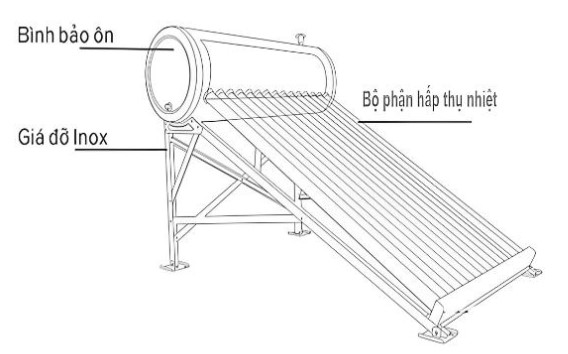
\includegraphics[width=0.6\linewidth]{../figs/D12-4-3}
	}
	Hỏi diện tích của phần góp là bao nhiêu mét vuông khi cần nâng nhiệt độ của 200 lít nước trong bình chứa từ $\SI{20}{\celsius}$ đến $\SI{40}{\celsius}$ trong 1 giờ. Biết khối lượng riêng của nước là $\SI{1000}{\kilogram/\meter^3}$; nhiệt dung riêng của nước là $\SI{4190}{\joule/\kilogram\cdot\kelvin}$; cường độ của ánh sáng Mặt Trời tới là $\SI{700}{\watt/\meter^2}$. \textit{(Kết quả lấy đến một chữ số sau dấu phẩy thập phân)}
	\shortans{33,3 }
	\loigiai{
		Nhiệt lượng cần thiết để làm nóng nước:
	$$Q=mc\Delta t=DVc\Delta t=\SI{16.76E6}{\joule}$$
	Năng lượng cần nhận từ Mặt Trời:
	$$W=\dfrac{Q}{H}=	\SI{83.8E6}{\joule}.$$
	Diện tích phần góp:
	$$\dfrac{W}{t}=IS\Rightarrow S\approx\SI{33.3}{\meter^2}.$$
	
	}
\end{ex}
% ===============================================================
\begin{ex}
	Đầu thép của một búa máy có khối lượng $\SI{10}{\kilogram}$ nóng lên thêm $\SI{20}{\celsius}$ sau 2 phút hoạt động. Biết rằng chỉ có $\SI{50}{\percent}$ cơ năng của búa máy chuyển thành nhiệt năng của đầu búa. Lấy nhiệt dung riêng của thép là $\SI{460}{\joule/\kilogram\cdot\kelvin}$. Công suất của búa bằng bao nhiêu $\si{\kilo\watt}$? \textit{(Kết quả lấy đến một chữ số sau dấu phẩy thập phân)}.
	\shortans{1,5 }
	\loigiai{
	Nhiệt lượng làm nóng đầu búa máy:
	$$Q=mc\Delta t=\SI{92000}{\joule}.$$
	Công suất búa máy:
	$$\calP=\dfrac{Q}{Ht}\approx\SI{1.5}{\kilo\watt}.$$
	}
\end{ex}
% ===============================================================
\begin{ex}
	Một ấm nước bằng kim loại có khối lượng $\SI{300}{\gram}$ và chứa 2 lít nước. Khi nhận được nhiệt lượng $\SI{517.44}{\kilo\joule}$, nhiệt độ của ấm và nước tăng từ $\SI{20}{\celsius}$ lên $\SI{80}{\celsius}$. Biết nhiệt dung riêng của nước là $\SI{4180}{\joule/\kilogram\cdot\kelvin}$, khối lượng riêng của nước là $\SI{1000}{\kilogram/\meter^3}$. Nhiệt dung riêng của kim loại làm ấm bằng bao nhiêu $\si{\joule/\kilogram\cdot\kelvin}$?
	\shortans{880 }
	\loigiai{
		$$Q=\left(m_nc_n+m_ac_a\right)\Delta t\Rightarrow c_a=\SI{880}{\joule/\kilogram\cdot\kelvin}.$$
	}
\end{ex}

\Closesolutionfile{ans}
\begin{center}
	\textbf{-- HẾT --}
\end{center}